%-------------------------------------------------------------------------------
\section{Alternatives to \cgroups{}}\label{s:alternatives}
%-------------------------------------------------------------------------------

Weights remains the \cgroups{} interface of choice for Kubernetes as well as
others like Firecracker and libvirt, but Linux also supports other mechanisms
for scheduling. In this section we discuss the existing alternatives to using
\cgroups{} weights in Linux, and show that none of them completely address the
issue.

The Linux scheduler is hierarchical: it supports different \textit{scheduling
classes}, within which there might be different \textit{policies}. The
\normalclass{} scheduling class is the one most people know --- it used to run a
Completely Fair Scheduler (CFS) and now runs a version of Earliest Eligible
Virtual Deadline First (EEVDF). It is the default scheduler, and \cgroups{}
weight is only effective within the \normalclass{} class.

\subsection{\schedidle{}}

\begin{figure}[t]
    \centering
    \begin{subfigure}[t]{\columnwidth}
        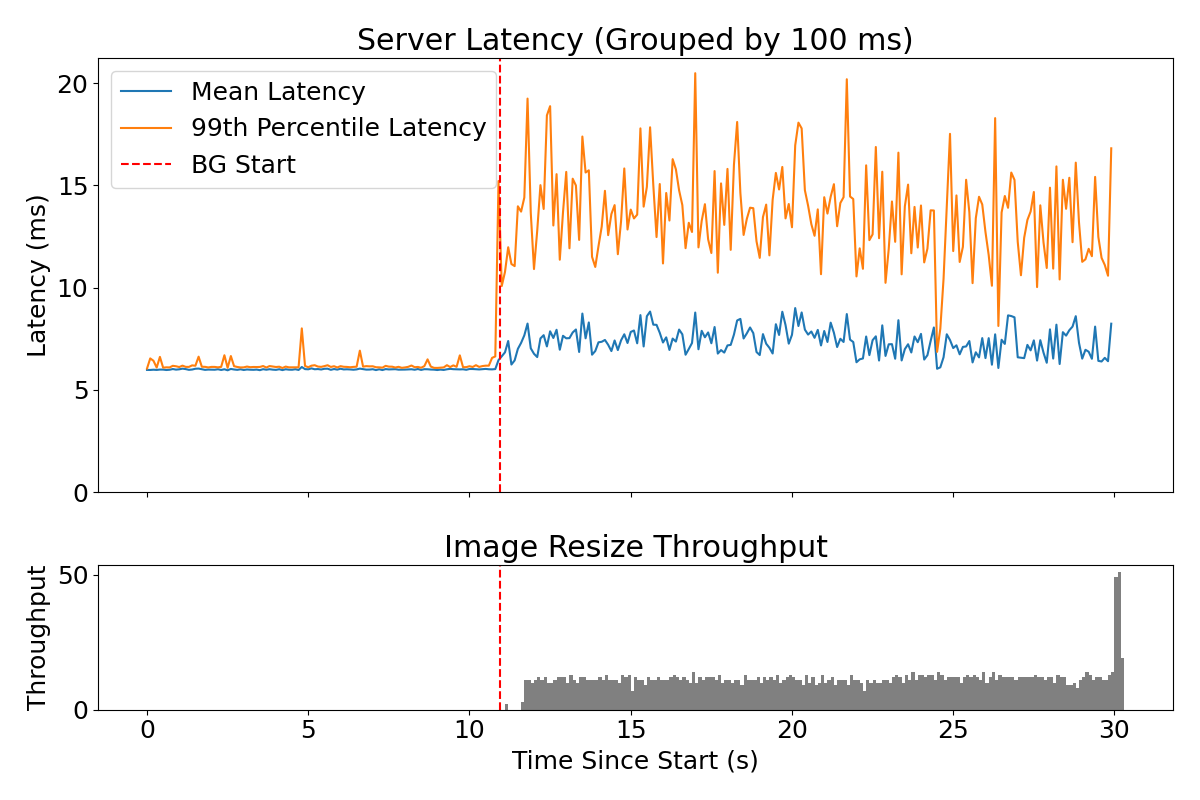
\includegraphics[width=\columnwidth]{graphs/srv-bg-idle-low.png}
        \caption{\schedidle{} in low load (85\%)}\label{fig:srv-bg-idle-low}
        \vspace{12pt}
    \end{subfigure}
    \hspace{\fill}
    \begin{subfigure}[t]{\columnwidth}
        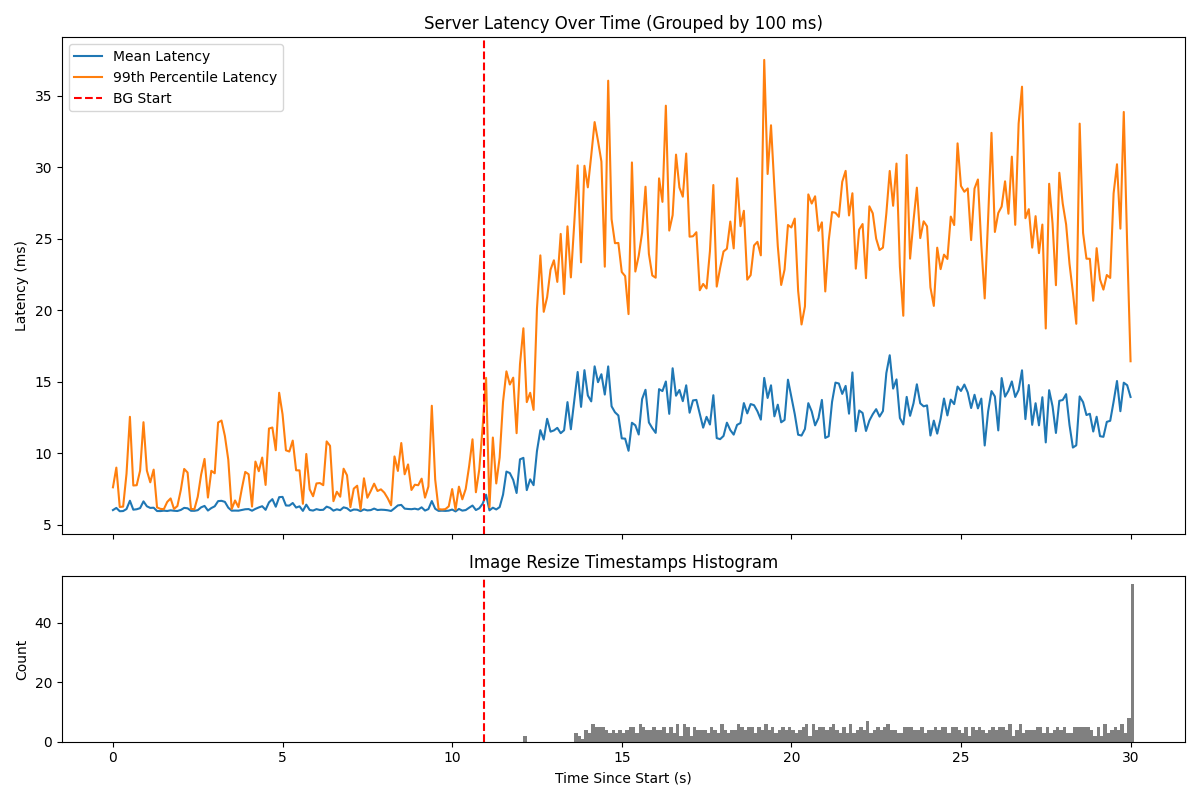
\includegraphics[width=\columnwidth]{graphs/srv-bg-idle-high.png}
        \caption{\schedidle{} in high load (95\%)}\label{fig:srv-bg-idle-high}
        \vspace{12pt}
    \end{subfigure}
    \vspace{4pt}
    \caption{}\label{fig:srv-bg-idle}
\end{figure}

\schedidle{} is Linux's current answer to doing a better job of separating best
effort tasks from those with reservations.

\schedidle{} is a scheduling policy that lives within the \normalclass{} class
alongside the default policy, which is \schednormal{}.\footnote{There is,
confusingly, also an Idle scheduling \textit{class}, but that is inaccessible to
userspace and exists solely to manage the core's transition in and out of being
actually idle (\ie{} running nothing).} 

Linux developers have improved \schedidle{} over the years, and it is meant to
support best effort workloads. It was also recently extended to have a
\cgroups{} interface file ~\cite{lkml-idle-cgroup}, so setting cpu.idle to
contain 1 puts the whole group under the \schedidle{} policy.

To determine whether \schedidle{} solves the problem with \cgroups{} weights, we
run the same microbenchmark, using \schedidle{} for the image resize job instead
of using a low \cgroups{} weight; \autoref{fig:srv-bg-idle} shows the results.


\subsection{Other scheduling classes}


\begin{figure}[t]
    \centering
    \begin{subfigure}[t]{\columnwidth}
        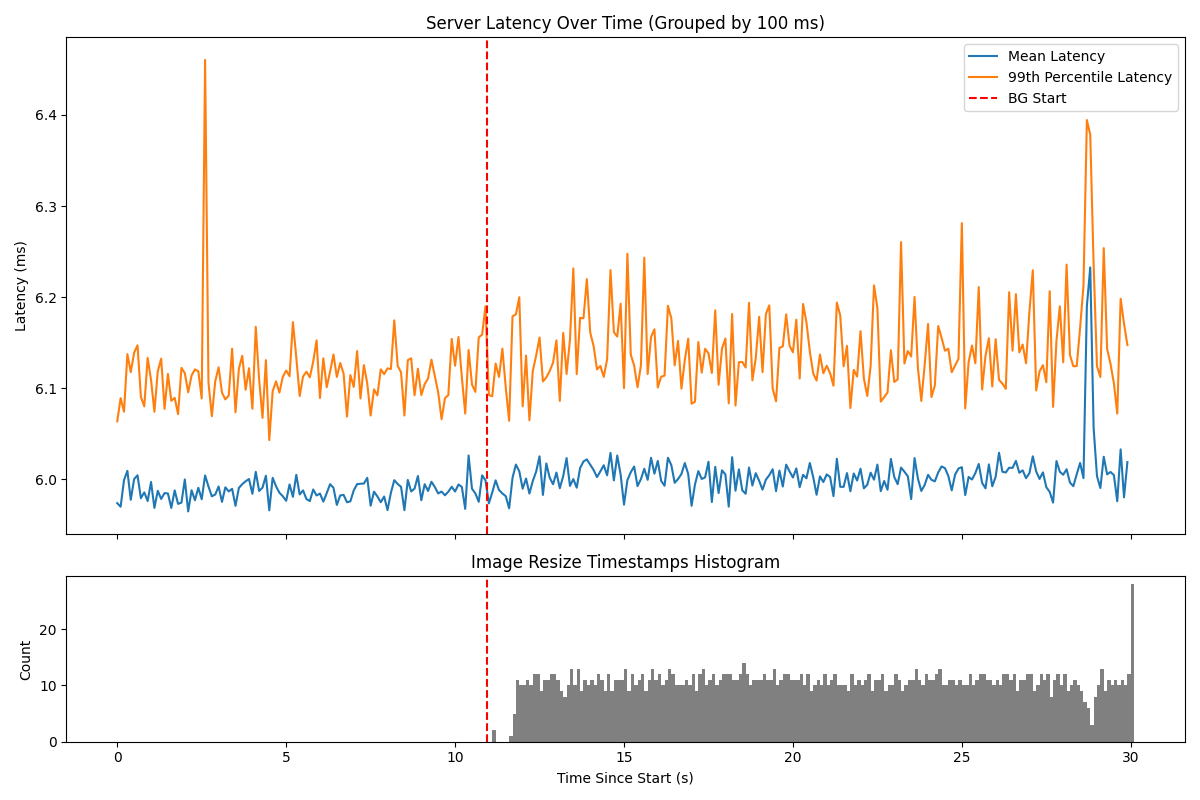
\includegraphics[width=\columnwidth]{graphs/srv-bg-rt-low.png}
        \caption{Low load (85\%)}\label{fig:srv-bg-rt-low}
        \vspace{12pt}
    \end{subfigure}
    \hspace{\fill}
    \begin{subfigure}[t]{\columnwidth}
        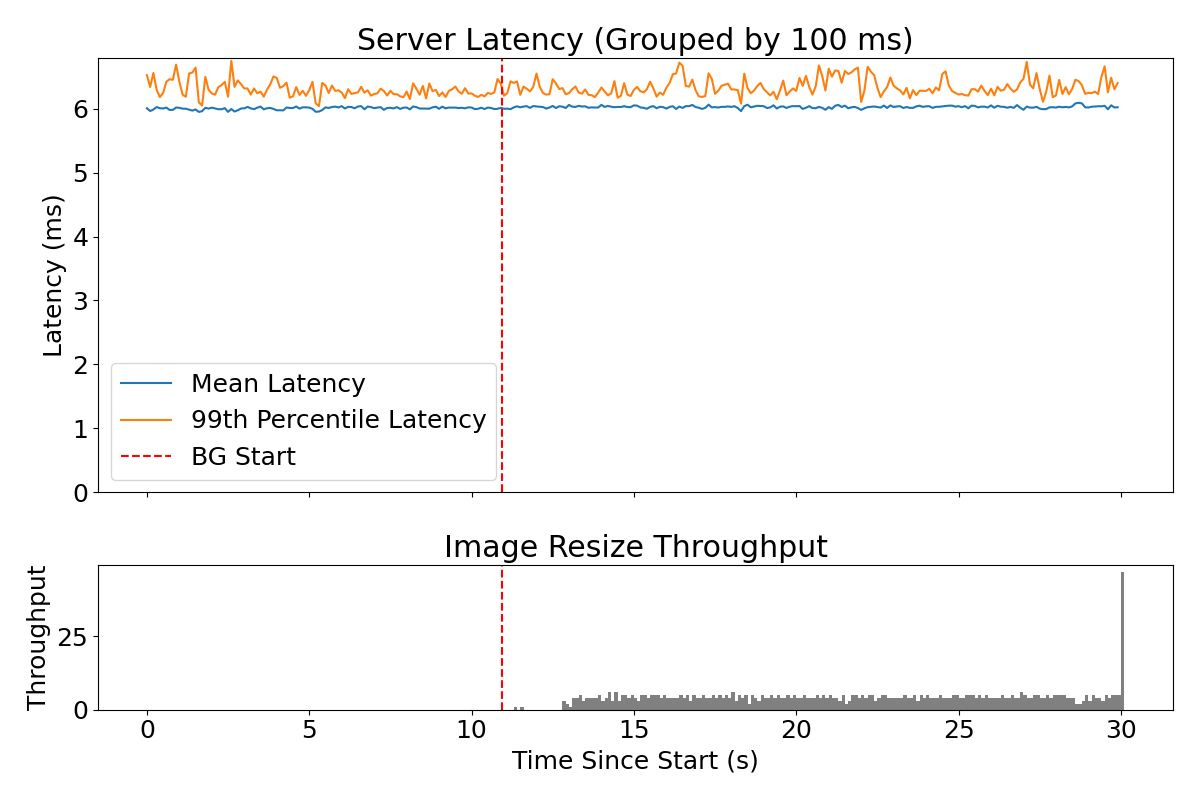
\includegraphics[width=\columnwidth]{graphs/srv-bg-rt-high.png}
        \caption{High load (95\%)}\label{fig:srv-bg-rt-high}
    \end{subfigure}
    \vspace{4pt}
    \caption{when running the server as a real time application, Linux does a
     good job of isolating the server's latencies from the load from best effort
     jobs }\label{fig:srv-bg-rt}
\end{figure}


Beyond \normalclass{}, the other two scheduling classes that are available to
users are \deadlineclass{} and \rtclass{}, both of which are designed to support
real-time applications.

These classes exist completely independently from one another: classes maintain
their own runqueues and per-entity state; implement their own scheduling
algorithms to choose from the entities on their runqueue; and balance the load
across runqueues on different cores.

Given that the desired behavior is strong separation between best effort
processes and those with reserved resources, using separate scheduling classes
for the two is an attractive proposition. 

The \deadlineclass{} scheduling class is not a good fit for running
microservices, since it requires accurate knowledge of a processes runtime
(processing time per request) and period (when requests come in). These are
neither fixed nor known ahead of time in many applications. 

The \rtclass{} has no such requirements for processes running in it, and allows
for oversubscription. \autoref{fig:srv-bg-rt} shows the result of running the
microbenchmark, but with the server running in the \rtclass{} scheduling class.
We can see that in both load settings the tail and average latency stays stable
at $\sim$6.0ms after starting the BE workload. The throughput of the image
resize job (10 iter/100ms at low load, and 5iter at high load) is around 80\% of
what it was in \autoref{fig:srv-bg-weight} when running the server with
\cgroups{} weights.


However, we show that the schedulers within each priority are not suited for
microservices (\autoref{sss:approch:linux:policies}), and that Linux method of
avoiding starvation has adverse effects on the LC application
(\autoref{sss:approach:linux:starve-throttle}).

\subsubsection{Real time schedulers are unsuitable for microservice
workloads}\label{sss:approch:linux:policies}

Running a microservice in \rtclass{} is untenable because of \rtclass{}'s
intra-priority schedulers. \rtclass{} has two different scheduling policies:
\schedfifo{} and \schedrr{}. Both have 99 priorities between which they enforce
strict priority; within priorities they differ in the policy they enforce.

\schedfifo{} uses first-in first-out run-to-completion scheduling. This means
that within each class, the process to run next will be the one that woke up
first, and it will run until it blocks or exits. When a blocked thread becomes
runnable again, that is counted as a wakeup and it will be put on the back of
the queue. This is known to have a failure mode of head-of-line (HoL) blocking
under varied request processing times, where long-running requests monopolize
the CPU while short requests wait in the queue.

\schedrr{} addresses this concern by running a round-robin scheduler that will
ensure Processor Sharing within each priority. Every thread just gets the same
scheduling quantum and then gets put at the end of that priority's queue. This
means that within each priority CPU time is allocated based on the number of
runnable threads. This conflicts with how weights are used within runqueues to
allocate CPU time between different LC workloads. Kubernetes, for instance,
allows users to make fractional CPU requests, which are enforced using weights.
Although \cgroups{} limits (\ie{} defining a maximum amount of runtime per
period each group can get) can also be applied to groups in real time
applications, Kubernetes requires the weight interface to allow for Burstable
pods.

\subsubsection{Linux throttles \rtclass{} processes under high load
}\label{sss:approach:linux:starve-throttle}

Schedulers running priority scheduling have to contend with the possibility of
starvation. Starvation can have many negative effects: it can cause deadlocks if
a low and high priority process share a lock (either in user-space or in
kernel-space), TCP connections can die while the process is being starved, and
it can miss interrupts like timers or completed i/o requests.

To avoid these, Linux chooses to ensure that no process is ever starved, which
it does by throttling high class processes with high load. Linux has two
different safeguards that enforce that no process is ever starved. One is that
\rtclass{} is as a scheduling class rate-limited: there are tuneable parameters
\texttt{sched\_rt\_runtime} and \texttt{sched\_rt\_period}, that together define
a rate limit for the \rtclass{} as a whole. The other safegaurd is that, even
when set to be equal (\ie{} \rtclass{} gets the full runtime each period if it
wants), the \normalclass{} scheduling class also has a so-called
\textit{deadline server}, which ensures it gets a small amount of time. The
deadline server is a `process' is in the \deadlineclass{} scheduling class with
a small amount of runtime per period, then when chosen will pass control on to
the \normalclass{} scheduler~\cite{lkml-deadline-srv}.

The throttling Linux chooses to do interferes with the goal of honoring
reservations, because it throttles the LC experiencing high load, which is
precisly when it needs its full reservation  most.


\begin{figure}[t]
    \centering
    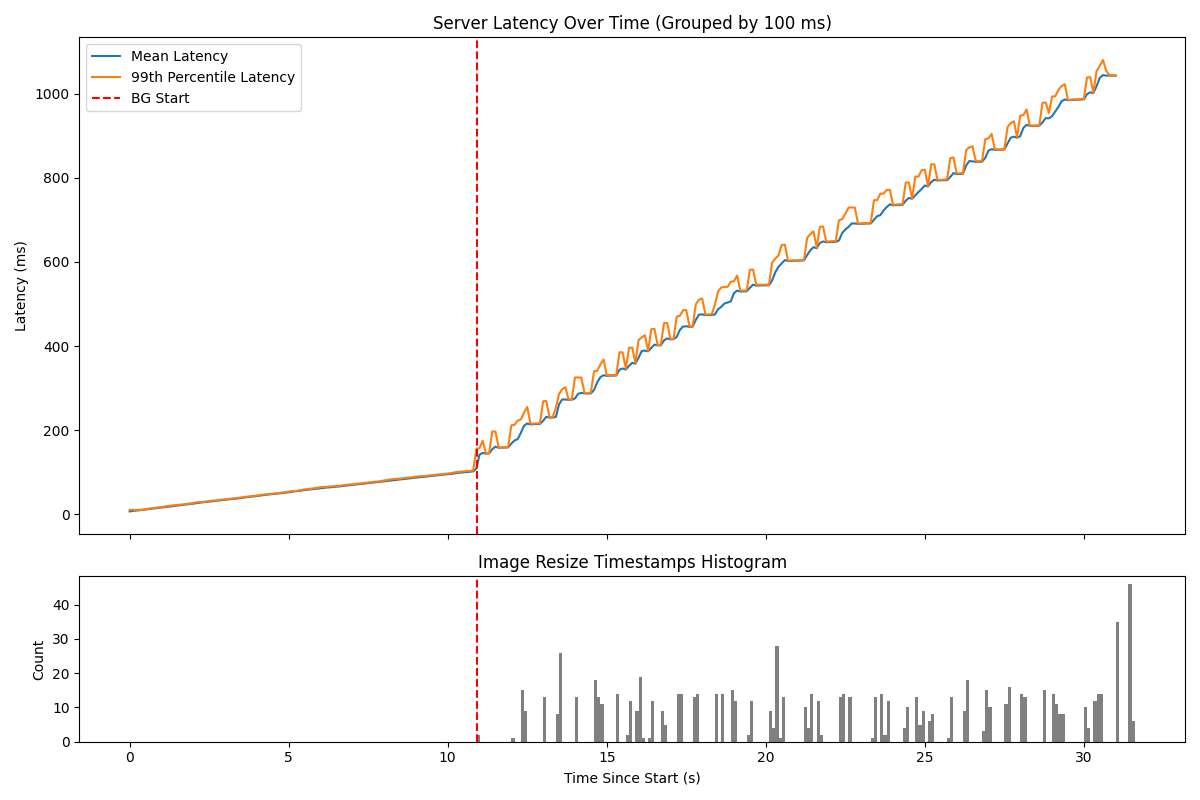
\includegraphics[width=\columnwidth]{graphs/overload-rt.png}
    \caption{LC in real time, throttling}\label{fig:overload-rt}
\end{figure}

Doing so impacts the performance of processes in the \rtclass{} at high load. We
can see this happen when we run the same microbenchmark experiment at a much
higher baseline utilization ($\sim$ 100\%). The results are in
\autoref{fig:overload-rt}. We see spikes begin to appear after starting the
image resize job, as the \rtclass{} server gets throttled in favor of running
the BE task; we see parallel spikes in the BE's throughput in the bottom graph.
Notice also the increase of the slope of response times after starting the
background tasks, this happens as the client has to queue requests while all the
current connections are blocked on running requests.

We conclude that Linux's mechanism of scheduling classes can enforce
reservations effectively, but that existing scheduling classes use algorithms
that are not a good fit for modern workloads, and that Linux doesn't enforce
reservations under high load because it throttles high priority classes.


\hmng{TODO should probably talk about cpusets here}


